\newpage
\section{超声波接近传感器总体设计与检测原理}
\subsection{超声波接近传感器总体设计}
本设计针对生产线上检测钢化玻璃到位问题,设计了一种稳定性好、灵活性高、应用场景广的超声波接近传感器。
本设计的总体设计如图\ref{超声波接近传感器总体设计}所示,包括了超声波接近传感器的硬件设计、软件设计和实验设计。
\begin{figure}[ht]
	\centering
	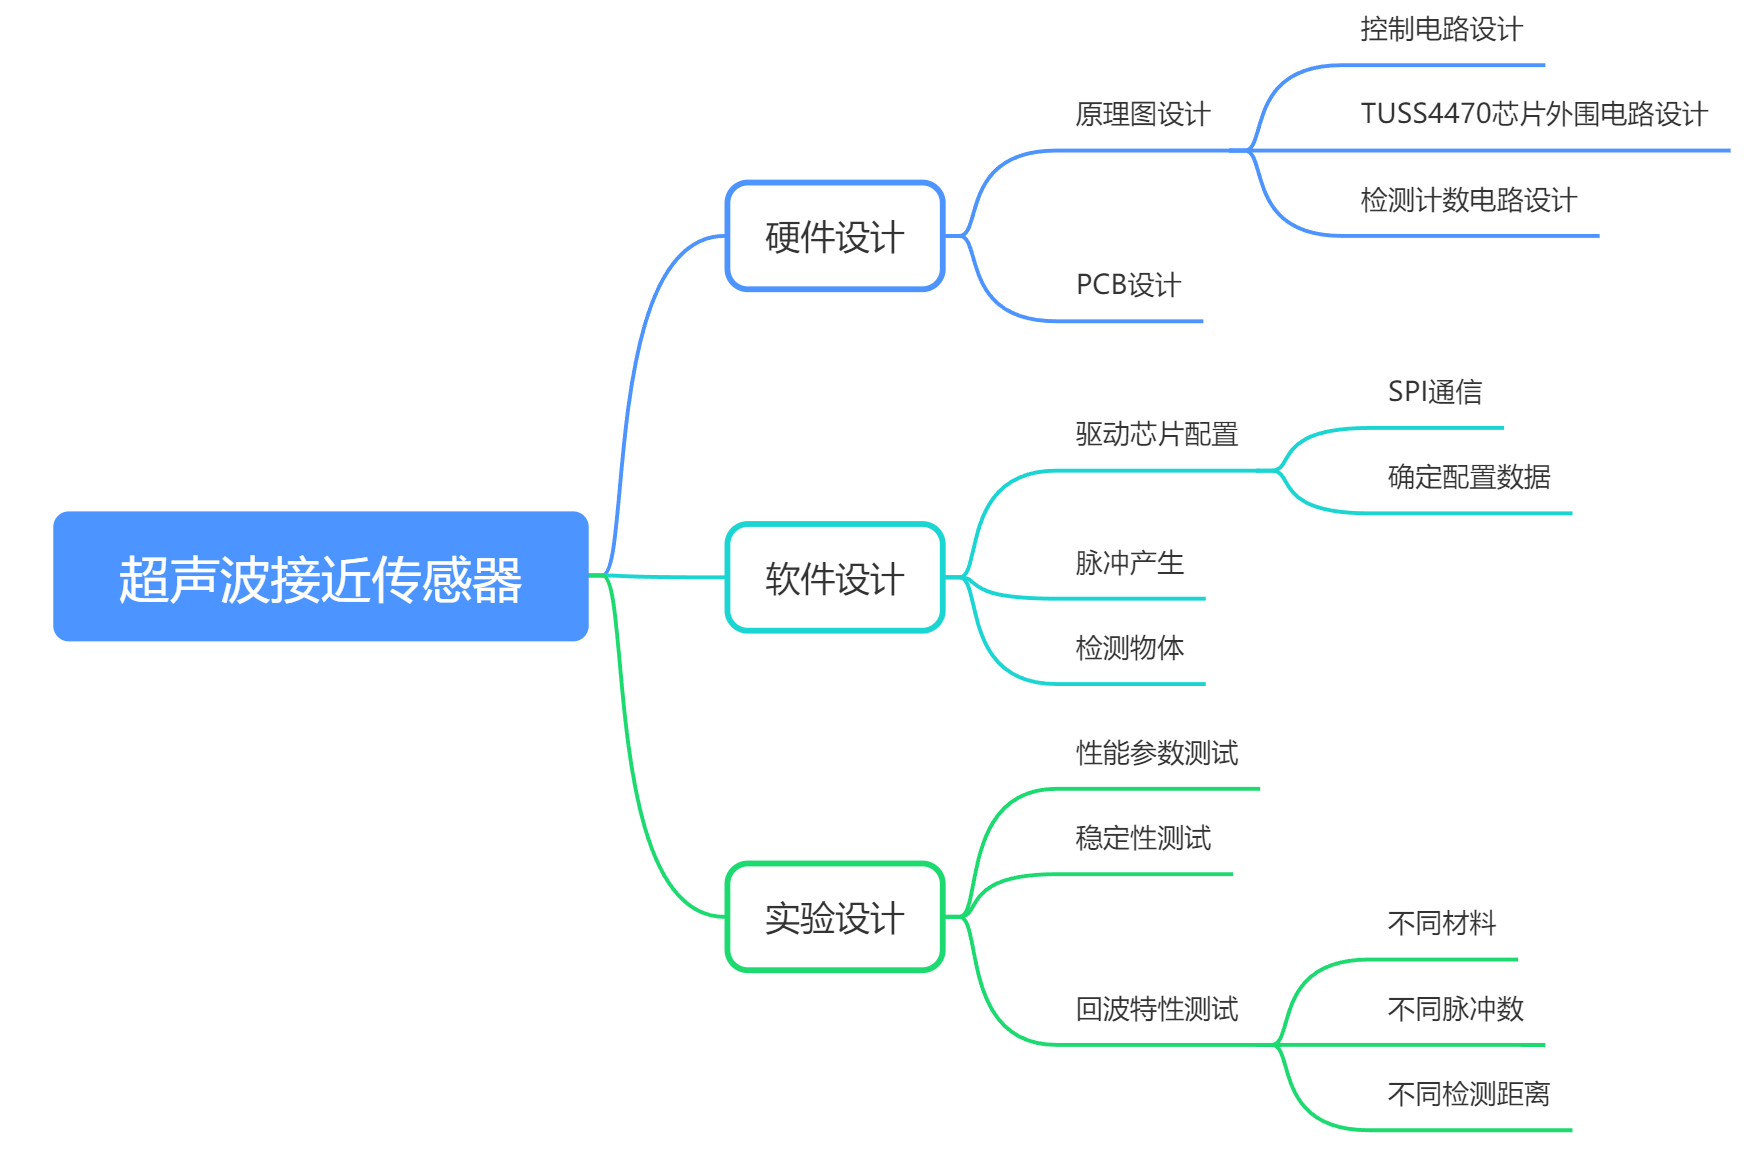
\includegraphics[width=12cm]{figure/overall designment.png}
	\caption{超声波接近传感器总体设计}
	\label{超声波接近传感器总体设计}
\end{figure}

硬件设计部分包括了原理图设计和PCB设计,软件设计包括了驱动芯片配置、脉冲信号产生、物体检测三个部分的程序设计,实验设计部分包括了设计实验进行性能参数测试、稳定性测试和回波特性测试。
\subsubsection{超声波接近传感器硬件设计}
硬件电路原理图的设计主要分为三部分来进行,分别为:超声波接近传感器控制电路设计、TUSS4470芯片外围电路设计、检测计数电路设计。其中超声波接近传感器控制电路的设计又包括了电源电路设计、时钟电路设计、JTAG下载电路设计、复位电路设计等。其中设计难度较大的是TUSS4470芯片外围电路,需要通过查阅芯片手册来完成各个引脚的设计。\par
硬件电路的PCB设计在传感器设计中同样有着重要的作用,对于TUSS4470芯片外围电路的PCB设计,芯片手册根据优先级给出了几大原则,用于减小各类信号相互之间的干扰,包括了电容、二极管等器件摆放位置优先级,分离接地,铺铜规则等。
\subsubsection{超声波接近传感器软件设计}
超声波接近传感器的软件设计根据功能分为了三个部分:芯片配置、脉冲产生、物体检测。\par
通过查找芯片手册,可以得知TUSS4470超声驱动芯片采用四线SPI协议来完成芯片配置,并与MCU进行通信,其采用的模式为CPOL=0、CPHA=1,即上升沿进行数据发送、下降沿进行数据接收,根据查找到的资料,本设计采用线性序列机(linear sequential machine)控制移位寄存器俩实现SPI通信。此外,SPI发送的各寄存器配置数据也需要参照芯片手册,根据应用场景进行确认。\par
在脉冲信号的模式选择上,考虑程序设计的难度以及运行速度,本设计选取脉冲模式3来产生脉冲控制信号,即以io2引脚输入的信号作为时钟信号,io1引脚的下降沿作为脉冲开始的触发信号,上升沿作为脉冲结束的触发信号。程序通过io1、io2引脚信号的下降沿进行触发计数,来得到脉冲信号的脉冲数以及发射次数。\par
物体检测部分程序主要功能为对回波信号进行处理判断。超声探头发出的脉冲波经物体反射后,重新被传感器所接收,回波信号通过TUSS4470芯片的解调放大处理后,变为简单的回波信号,程序按照检测逻辑对回波信号进行检测判断,从而控制检测状态的转移。
\subsubsection{超声波接近传感器实验设计}
在完成实物的制作与调试后,还需要设计实验来测试传感器的性能以及检测逻辑的可行性。\par
实验设计部分包括了设计实验测试超声波接近传感器性能参数、稳定性以及回波特性。性能参数测试包括了检测范围测试和精度测试,稳定性测试的目的在于测试传感器检测逻辑的必要性,回波特性测试则是为后续的应用提供参考。


\subsection{超声波接近传感器检测原理}
\begin{figure}[!h]
	\centering
	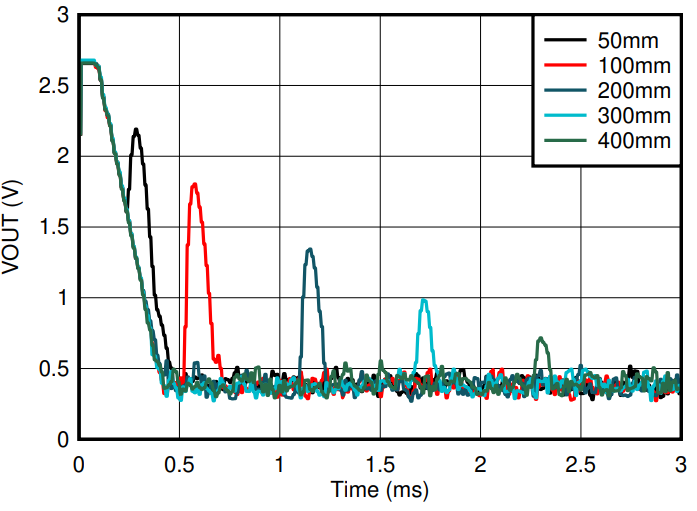
\includegraphics[width=8cm]{figure/VOUT image.png}
	\caption{VOUT输出\upcite{TUSS4470芯片手册}}
	\label{VOUT输出}
\end{figure}\par
通过查阅芯片手册\upcite{TUSS4470芯片手册},我们可以知道,TUSS4470芯片采用的检测原理为飞行时间法,获取飞行时间的方法为固定阈值法。\par
芯片通过滤波解调等处理,可将回波信号处理成一个简单的单峰信号,由VOUT引脚输出,当峰值超过所设定阈值时,即判定为超声换能器接收到回波,该峰值距离起点的时间随检测距离的变化而变化。如图\ref{VOUT输出}所示,当检测物体距离传感器$50mm$、$100mm$、$200mm$、$300mm$、$400mm$时,信号的峰值在不断减小,也在不断地向右侧进行移动。但是在到达有效波峰前,仍然存在着一个波峰信号,影响着物体的检测。通过查阅资料我们得知,这是由于压电振子存在的余振现象所导致的,自发自收的换能器在接收到反射回波时,发射脉冲的余振尚未消失,从而产生一段不能检测回波信号的“盲区”。\par
波峰距离起点的时间$t$由以下公式得出:       
\begin{align}
	t&=t_1+t_2+t_3 \\
	t&_2=\frac{D}{c}
	\label{检测周期公式}
\end{align}  
式中\quad$t$---波峰距离起点时间;\par
\quad$t_1$---脉冲余振时间;\par
\quad$t_2$---飞行时间;\par    
\quad$t_3$---芯片处理回波所花费时间;\par 
\quad$D$---检测物体距离传感器的距离;\par  
\quad$c$---声波在空气中的传播速度\par    
根据任务书中的要求,超声波接近传感器的检测范围为$100mm\sim200mm$,为简化程序,我们通过设定检测窗口的方式来实现该效果。\par  
当物体与传感器的距离确定时,回波信号波峰对应的$t$也是确定的,该值可以通过实验测得。例如距离为$100mm$、$200mm$时,对应$t$为$1.2ms$、$2.4ms$,那么我们可以设定检测窗口为$1.2ms\sim2.4ms$,只对这个范围内的波峰进行检测,而屏蔽范围外的信号,从而避免被“盲区”信号所干扰,并且实现检测$100mm\sim200mm$范围物体的功能。\par
